\documentclass[notes, 12.5pt, aspectratio=169]{beamer}

\usepackage{pgfpages}
\usepackage{threeparttable}
% These slides also contain speaker notes. You can print just the slides,
% just the notes, or both, depending on the setting below. Comment out the want
% you want.

\setbeameroption{hide notes} % Only slide
%\setbeameroption{show only notes} % Only notes
%\setbeameroption{show notes on second screen=right} % Both


%fonts
%\usepackage{bookman}
%\usepackage[default]{lato}
%\usepackage{helvet}
\usepackage[sc]{mathpazo}
%\usepackage{tex-gyre}


\usepackage{array}
\usepackage{bm}


\usepackage{tikz}
\usepackage{verbatim}
\setbeamertemplate{note page}{\pagecolor{yellow!5}\insertnote}
\usetikzlibrary{positioning}
\usetikzlibrary{snakes}
\usetikzlibrary{calc}
\usetikzlibrary{arrows}
\usetikzlibrary{decorations.markings}
\usetikzlibrary{shapes.misc}
\usetikzlibrary{matrix,shapes,arrows,fit,tikzmark}
\usepackage{amsmath}
\usepackage{mathpazo}
\usepackage{hyperref}
\usepackage{lipsum}
\usepackage{multimedia}
\usepackage{graphicx}
\usepackage{multirow}
\usepackage{graphicx}
\usepackage{dcolumn}
%\usepackage{enumitem}
\usepackage{bbm}
\newcolumntype{d}[0]{D{.}{.}{5}}


\usepackage[backend=biber, style=authoryear, citestyle=authoryear, uniquename=false, firstinits=true, maxbibnames=5, minbibnames=1, maxcitenames=2, mincitenames=1, uniquelist=false, datelabel=short, labeldate=year, alldates=year]{biblatex}
\addbibresource{lib_parenting_styles.bib}

\usepackage{changepage}
\usepackage{appendixnumberbeamer}
\newcommand{\beginbackup}{
   \newcounter{framenumbervorappendix}
   \setcounter{framenumbervorappendix}{\value{framenumber}}
   \setbeamertemplate{footline}
   {
     \leavevmode%
     \hline
     box{%
       \begin{beamercolorbox}[wd=\paperwidth,ht=2.25ex,dp=1ex,right]{footlinecolor}%
%         \insertframenumber  \hspace*{2ex} 
       \end{beamercolorbox}}%
     \vskip0pt%
   }
 }
\newcommand{\backupefnd}{
   \addtocounter{framenumbervorappendix}{-\value{framenumber}}
   \addtocounter{framenumber}{\value{framenumbervorappendix}} 
}


\usepackage{graphicx}
\usepackage[space]{grffile}
\usepackage{booktabs}

% These are my colors -- there are many like them, but these ones are mine.
\definecolor{blue}{RGB}{0,114,178}
\definecolor{red}{RGB}{213,94,0}
\definecolor{yellow}{RGB}{240,228,66}
\definecolor{green}{RGB}{0,158,115}

\hypersetup{
  colorlinks=true,
  linkbordercolor = {white},
  linkcolor = {blue}
}


%% I use a beige off white for my background
\definecolor{MyBackground}{RGB}{255,253,218}

%% Uncomment this if you want to change the background color to something else
%\setbeamercolor{background canvas}{bg=MyBackground}

%% Change the bg color to adjust your transition slide background color!
\newenvironment{transitionframe}{
  \setbeamercolor{background canvas}{bg=white}
  \begin{frame}}{
    \end{frame}
}

\setbeamercolor{frametitle}{fg=blue}
\setbeamercolor{title}{fg=black}
\setbeamertemplate{footline}[frame number]
\setbeamertemplate{navigation symbols}{} 
\setbeamertemplate{itemize items}{-}
\setbeamercolor{itemize item}{fg=blue}
\setbeamercolor{itemize subitem}{fg=blue}
\setbeamercolor{enumerate item}{fg=blue}
\setbeamercolor{enumerate subitem}{fg=blue}
\setbeamercolor{button}{bg=MyBackground,fg=blue,}



% If you like road maps, rather than having clutter at the top, have a roadmap show up at the end of each section 
% (and after your introduction)
% Uncomment this is if you want the roadmap!
 \AtBeginSection[]
 {
    \begin{frame}
        \frametitle{Roadmap}
        \tableofcontents[currentsection]
    \end{frame}
 }
\setbeamercolor{section in toc}{fg=blue}
\setbeamercolor{subsection in toc}{fg=red}
\setbeamersize{text margin left=1em,text margin right=1em} 

\newenvironment{wideitemize}{itemize\addtolength{\itemsep}{10pt}}{\enditemize}

\usepackage{environ}
\NewEnviron{videoframe}[1]{
  \begin{frame}
    \vspace{-8pt}
    \begin{columns}[onlytextwidth, T] % align columns
      \begin{column}{.58\textwidth}
        \begin{minipage}[t][\textheight][t]
          {\dimexpr\textwidth}
          \vspace{8pt}
          \hspace{4pt} {\Large \sc \textcolor{blue}{#1}}
          \vspace{8pt}
          
          \BODY
        \end{minipage}
      \end{column}%
      \hfill%
      \begin{column}{.42\textwidth}
        \colorbox{green!20}{\begin{minipage}[t][1.2\textheight][t]
            {\dimexpr\textwidth}
            Face goes here
          \end{minipage}}
      \end{column}%
    \end{columns}
  \end{frame}
}


\makeatletter
\newcommand{\fitimage}[2][\@nil]{
	\begin{figure}
		\begin{adjustbox}{width=0.9\textwidth, totalheight=\textheight-2\baselineskip-2\baselineskip,keepaspectratio}
			\includegraphics{#2}
		\end{adjustbox}
		\def\tmp{#1}%
		\ifx\tmp\@nnil
		\else
		\caption{#1}
		\fi
	\end{figure}
}
\makeatother

\newcommand{\be}{\bm{\beta}}
\newcommand{\x}{\textbf{x}}
\newcommand{\z}{\textbf{z}}
\newcommand{\X}{\textbf{X}}
\newcommand{\Y}{\textbf{Y}}


\title[]{\textcolor{blue}{TBA}}
\author[PGP]{}
\institute[ifo]{\small{\begin{tabular}{c c}
\large Florian Schoner   \\
\large ifo  \\
\end{tabular}}}

\date{\today}


\begin{document}

%%% TIKZ STUFF
\tikzset{   
        every picture/.style={remember picture,baseline},
        every node/.style={anchor=base,align=center,outer sep=1.5pt},
        every path/.style={thick},
        }
\newcommand\marktopleft[1]{%
    \tikz[overlay,remember picture] 
        \node (marker-#1-a) at (-.3em,.3em) {};%
}
\newcommand\markbottomright[2]{%
    \tikz[overlay,remember picture] 
        \node (marker-#1-b) at (0em,0em) {};%
}
\tikzstyle{every picture}+=[remember picture] 
\tikzstyle{mybox} =[draw=black, very thick, rectangle, inner sep=10pt, inner ysep=20pt]
\tikzstyle{fancytitle} =[draw=black,fill=red, text=white]
%%%% END TIKZ STUFF

% Title Slide
\begin{frame}
\maketitle
  %\centering The views expressed do not necessarily reflect the position of the Federal Reserve Bank of New York or the Federal Reserve System.
\end{frame}





\section{Motivation}
%\begin{transitionframe}
%  \begin{center}
%    { \Huge \textcolor{black}{Spacing and Words}}
%  \end{center}
%\end{transitionframe}
\begin{frame}{Motivation}
	\centering
	\begin{columns}
	\begin{column}{1\textwidth}
		\only<1>{\resizebox{0.8\textwidth}{!}{
				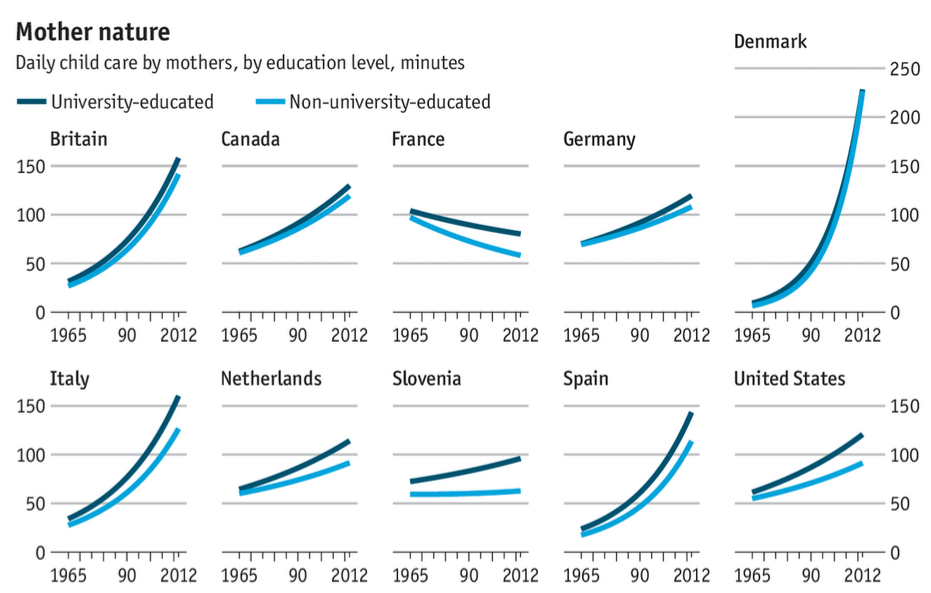
\includegraphics{maternal_time_investments.png}
			}
		}
	\end{column}
	\end{columns}
	\begin{itemize}[(I)]
		\item<2-> Parental (time) investments are an important input to children's technology of skill formation \parencites{falkSocioEconomicStatusInequalities2021}{attanasioEstimatingProductionFunction2020}
		\item<3-> Recent literature emphasizes that parents choose sets of behaviors, ``\textit{parenting styles}'' \parencite{baumrindChildCarePractices1967} of which time investments and their productivity are merely one aspect (\cite{doepkeParentingStyleAltruism2017, doepkeEconomicsParenting2019, cobb-clarkParentingStyleInvestment2019}).
		\item<4-> Little is known how parenting styles can be measured empirically \parencites{chanParentingStyleYouth2011}{rauhParentingTypes2020}
		%maybe motivate this with a graph that more educated parents spend more time w/ their children? -> What do they do with their children in that time?! Time trends
	\end{itemize}
\end{frame}
%
\begin{frame}{This paper}
	\begin{itemize}[(I)]
		\item<1-> Research Question: How can we measure parenting styles and its determinants empirically?
		\item[]<2->$\Longrightarrow$ Requires two things:
		\begin{enumerate}
			\item<3-> Data-driven identification of (latent) parenting styles $\rightarrow$ Gaussian Mixture Model \parencite{hastieElementsStatisticalLearning2009}
			\item<4-> Which parental characteristics predict the choice of parenting styles identified in 1?
		\end{enumerate}
		\item<5-> Data: German National Educational Panel Study \parencite{nepsnationaleducationalpanelstudybamberggermanyNEPSStartingCohort2021}
		\item<6-> Results
		\begin{enumerate}
			\item<6-> 3 parenting styles 
			\item<7-> Parental time investment best predicts the choice of a parenting style
		\end{enumerate}
	\end{itemize}
\end{frame}

\section{Data}
\begin{frame}{Data}
	\begin{itemize}[(I)]
		\item<1-> Panel of 3481 newborns; focus on children's environment and competence development
		\item<2-> 3 main types of data
		\begin{enumerate}
			\item<3-> Measures of \textbf{parenting styles} ask how often typical situations occur between parent and child.
			\item<4-> Measures of \textbf{interaction behaviors} are derived from videotaped recordings of a parent-child play scene
			\item<5-> Family and child characteristics
		\end{enumerate}
	\end{itemize}
\end{frame}


\section{Classification}
\begin{frame}{Classification: Gaussian Mixture Model}
	\begin{itemize}[(I)]
		\item<1-> Assume that vector of scores of parenting styles, $\bm{x}_i$, $i=1,\ldots,N$ is drawn from a mixture of multivariate normal densities and estimate their parameters
		\item[]<2-> \begin{equation*} f(x) = \sum_{m=1}^{M} \alpha_m \phi(x; \mu_m, \bm{\Sigma}_m) \end{equation*}
		\item<3-> Assign observation to the class (density) with the best-fitting parameters \begin{equation*}
			\max_{1 \leqslant m \leqslant M} \widehat{\text{Pr}}(i \in m) = \frac{\widehat{\alpha}_m \phi(x_i; \widehat{\mu}_m, \widehat{\bm{\Sigma}}_m)}{\sum_{k=1}^{M} \widehat{\alpha}_k \phi(x_i; \widehat{\mu}_k, \widehat{\bm{\Sigma}}_k)}
		\end{equation*}
	\item<4-> Gives assignment probabilities for all classes $\rightsquigarrow$ uncertainty measure
	\end{itemize}
\end{frame}

\section{Results}
\begin{frame}{Results: Classification}
	\makebox[\linewidth][c]{
		\begin{threeparttable}
		\begin{tabular}{lcccccc}
			\hline \hline\\[-1.8ex] 
			&    &    &    &\multicolumn{3}{c}{p-values} \\ 
			\cline{5-7} \\[-1.8ex]Dimension & 1 & 2 & 3 & 1/2 & 1/3 & 2/3 \\ 
			\midrule
			Powerful enforcement & \marktopleft{a1}0.033 & 0.057 & -0.066 \markbottomright{a1}{red} & 0.596 & 0.001 & 0.004 \\ 
			Emotional warmth & 0.130 & 0.370 & -0.241 & 0.000 & 0.000 & 0.000 \\ 
			Inconsistent parent. & -0.101 & -0.095 & 0.112 & 0.641 & 0.000 & 0.000 \\ 
			Neg. communication & -0.076 & -0.235 & 0.177 & 0.000 & 0.000 & 0.000 \\ 
			Monitoring & \marktopleft{a2} 0.099 & 0.290 & -0.199 \markbottomright{a2}{red}& 0.000 & 0.000 & 0.000 \\ 
			Autonomy & \marktopleft{a3}-0.007 & 0.191 & -0.066 \markbottomright{a3}{red}& 0.000 & 0.000 & 0.000 \\ 
			Pos. parent. behavior & -0.097 & 0.669 & -0.136 & 0.000 & 0.485 & 0.000 \\ 
			%Psychological control & -0.127 & -0.100 & 0.137 & 0.178 & 0.000 & 0.000 \\ 
			\hline \bottomrule
		\end{tabular}
	\begin{tablenotes}
		\small
		\item \textit{Notes}: Class means of the different parenting styles dimensions based on $N = 1504$ observations. P-values for $t$-tests on equality of means against a two-sided alternative.
	\end{tablenotes}
	\end{threeparttable}
	}
\uncover<1-1>{\tikz[overlay,remember picture,inner sep=1pt]
	\node[draw=red,rounded corners,fit=(marker-a1-a.north west) (marker-a1-b.south east)] {};}
\uncover<2-2>{\tikz[overlay,remember picture,inner sep=1pt]
	\node[draw=red,rounded corners,fit=(marker-a2-a.north west) (marker-a2-b.south east)] {};}
\uncover<3-3>{\tikz[overlay,remember picture,inner sep=1pt]
	\node[draw=red,rounded corners,fit=(marker-a2-a.north west) (marker-a2-b.south east)] {};}
\end{frame}

\begin{frame}{Results: Multinomial Logit}
	\begin{itemize}[(I)]
		\item<1-> Do differences in parent-child interaction behavior and/or family characteristics predict the choice of parenting style?
		\item[]<2-> \begin{equation*} \text{Pr}(\text{parenting style}_i = m) = \frac{\exp(\x^\top_{i} \be_m + \z^\top_{i} \bm{\gamma}_m)}{\sum_{l=1}^{3} \exp(\x^\top_{i}\be_l + \z^\top_{i} \bm{\gamma}_l)}, \qquad m = 1, 2, 3, \label{eq:multinom}
		\end{equation*}
		\begin{itemize}
			\item <2-> $m$: either authoritative, authoritarian, or permissive
			\item <2-> $\x_i$ contains measures of parental interaction behavior
			\item <2-> $\z_i$ captures the child's socio-economic environment
		\end{itemize} 
	\end{itemize}
\end{frame}

\begin{frame}[fragile]{Change your fonts!}
  \begin{itemize}
  \item[-] Hi
  \item[-] Changing fonts is easy and productive
  \item[-] This slide deck uses Lato -- you can experiment!
  \item[-] Here's some comparison to alternatives:\\
    \begin{itemize}
    \item[]    {Lato: the \textit{quick} \textbf{brown} fox jumps over the $\alpha$- dog}\\
    \item[]     {\fontfamily{cmr}\selectfont  Arial (default): the \textit{quick} \textbf{brown} fox jumps over the $\alpha$- dog}\\
    \item[]     {\fontfamily{pbk}\selectfont  Bookman: the \textit{quick} \textbf{brown} fox jumps over the $\alpha$- dog}\\
    \item[]     {\fontfamily{phv}\selectfont  Helvetica: the \textit{quick} \textbf{brown} fox jumps over the $\alpha$- dog}\\
    \end{itemize}
  \end{itemize}
  \bigskip
  To change your font globally, you'll need to find the right package:
  \begin{verbatim}
   \usepackage[default]{lato}
   \end{verbatim}
  Link for choices: \url{http://www.tug.dk/FontCatalogue/sansseriffonts.html}
\end{frame}

\begin{frame}[allowframebreaks]
	\printbibliography
\end{frame}

\section{Appendix}

\appendix

\begin{frame}[label=appendix_start]{Almost done!}
  \begin{itemize}
  \item See, now we're in backup slide land
  \item This is made useful by having links throughtout the talk
  \item Here's a button, which is how I make links \hyperlink{appendix_end}{\beamergotobutton{Next slide}}
  \end{itemize}
\end{frame}

\begin{frame}[label=appendix_end]{Use it to intimidate audiences!}
  \begin{itemize}
    \item[] Now you can make it clear you've done a shitload of work
      \begin{itemize}
      \item[]  without having to show everything! \hyperlink{appendix_start}{\beamergotobutton{Back}}
      \end{itemize}
    \item[] You label a frame with the \texttt{[label=name]} option, and then point a link to it
    \item[] You can make an object a link using the \texttt{\textbackslash hyperlink\{label\}\{object\}} command
  \end{itemize}
\end{frame}



\end{document}
